\documentclass{standalone}
\usepackage{tikz}
\usetikzlibrary{patterns, positioning}


\begin{document}
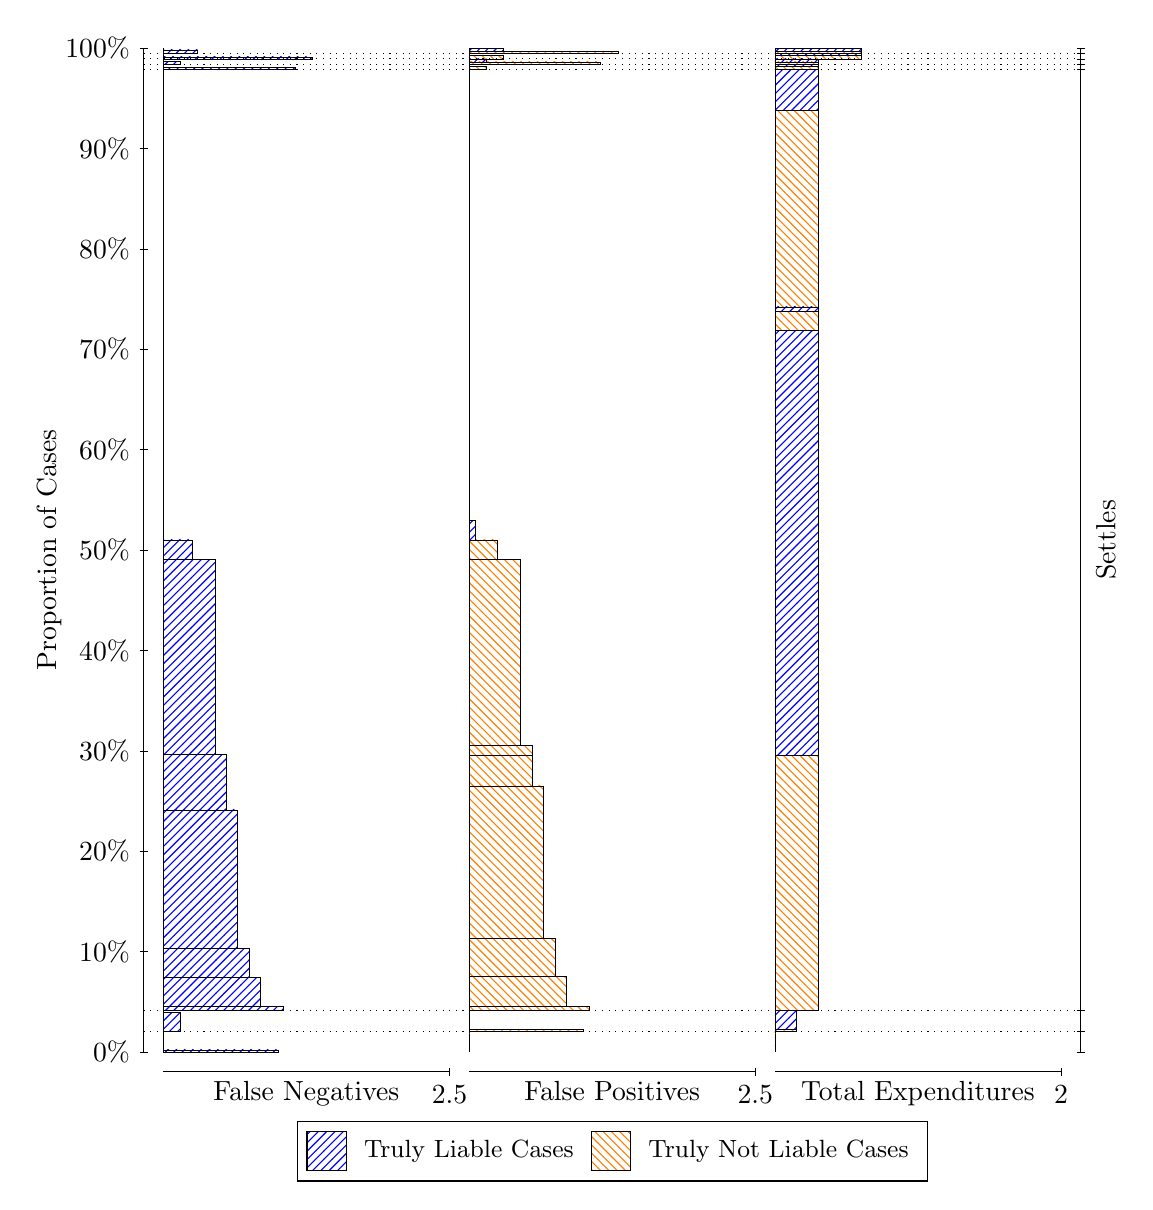
\begin{tikzpicture}
\draw[black, very thin] (1.5,1.75) -- (1.5,14.5);
\node[rotate=90, text=black, anchor=center] at (0.3, 8.125) {Proportion of Cases};
\draw[black, very thin] (1.45,1.75) -- (1.55,1.75);
\node[text=black, anchor=east] at (1.45, 1.75) {0\%};
\draw[black, very thin] (1.45,3.025) -- (1.55,3.025);
\node[text=black, anchor=east] at (1.45, 3.025) {10\%};
\draw[black, very thin] (1.45,4.3) -- (1.55,4.3);
\node[text=black, anchor=east] at (1.45, 4.3) {20\%};
\draw[black, very thin] (1.45,5.575) -- (1.55,5.575);
\node[text=black, anchor=east] at (1.45, 5.575) {30\%};
\draw[black, very thin] (1.45,6.85) -- (1.55,6.85);
\node[text=black, anchor=east] at (1.45, 6.85) {40\%};
\draw[black, very thin] (1.45,8.125) -- (1.55,8.125);
\node[text=black, anchor=east] at (1.45, 8.125) {50\%};
\draw[black, very thin] (1.45,9.4) -- (1.55,9.4);
\node[text=black, anchor=east] at (1.45, 9.4) {60\%};
\draw[black, very thin] (1.45,10.675) -- (1.55,10.675);
\node[text=black, anchor=east] at (1.45, 10.675) {70\%};
\draw[black, very thin] (1.45,11.95) -- (1.55,11.95);
\node[text=black, anchor=east] at (1.45, 11.95) {80\%};
\draw[black, very thin] (1.45,13.225) -- (1.55,13.225);
\node[text=black, anchor=east] at (1.45, 13.225) {90\%};
\draw[black, very thin] (1.45,14.5) -- (1.55,14.5);
\node[text=black, anchor=east] at (1.45, 14.5) {100\%};

\draw[black, very thin] (13.4,1.75) -- (13.4,14.5);
\draw[black, very thin] (13.35,1.75) -- (13.45,1.75);
\node[anchor=west] at (13.35, 1.75) {};
\draw[black, very thin] (13.35,2.0136) -- (13.45,2.0136);
\node[anchor=west] at (13.35, 2.0136) {};
\draw[black, very thin] (13.35,2.2772) -- (13.45,2.2772);
\node[anchor=west] at (13.35, 2.2772) {};
\draw[black, very thin] (13.35,14.229) -- (13.45,14.229);
\node[anchor=west] at (13.35, 14.229) {};
\draw[black, very thin] (13.35,14.294) -- (13.45,14.294);
\node[anchor=west] at (13.35, 14.294) {};
\draw[black, very thin] (13.35,14.363) -- (13.45,14.363);
\node[anchor=west] at (13.35, 14.363) {};
\draw[black, very thin] (13.35,14.432) -- (13.45,14.432);
\node[anchor=west] at (13.35, 14.432) {};
\draw[black, very thin] (13.35,14.5) -- (13.45,14.5);
\node[anchor=west] at (13.35, 14.5) {};

\draw[black, very thin, pattern color=blue, pattern=north east lines] (1.75,1.75) rectangle (3.2033,1.7777);
\draw[black, very thin, pattern color=orange, pattern=north west lines] (1.75,1.7777) rectangle (1.75,2.0136);
\draw[black, very thin, pattern color=blue, pattern=north east lines] (1.75,2.0136) rectangle (1.968,2.2494);
\draw[black, very thin, pattern color=orange, pattern=north west lines] (1.75,2.2494) rectangle (1.75,2.2772);
\draw[black, very thin, pattern color=blue, pattern=north east lines] (1.75,2.2772) rectangle (3.276,2.3311);
\draw[black, very thin, pattern color=blue, pattern=north east lines] (1.75,2.3311) rectangle (2.9853,2.6936);
\draw[black, very thin, pattern color=blue, pattern=north east lines] (1.75,2.6936) rectangle (2.84,3.0705);
\draw[black, very thin, pattern color=blue, pattern=north east lines] (1.75,3.0705) rectangle (2.6947,4.8231);
\draw[black, very thin, pattern color=blue, pattern=north east lines] (1.75,4.8231) rectangle (2.5493,5.5277);
\draw[black, very thin, pattern color=blue, pattern=north east lines] (1.75,5.5277) rectangle (2.404,8.0063);
\draw[black, very thin, pattern color=blue, pattern=north east lines] (1.75,8.0063) rectangle (2.1133,8.2521);
\draw[black, very thin, pattern color=orange, pattern=north west lines] (1.75,8.2521) rectangle (1.75,14.229);
\draw[black, very thin, pattern color=blue, pattern=north east lines] (1.75,14.229) rectangle (3.4213,14.257);
\draw[black, very thin, pattern color=orange, pattern=north west lines] (1.75,14.257) rectangle (1.75,14.294);
\draw[black, very thin, pattern color=blue, pattern=north east lines] (1.75,14.294) rectangle (1.968,14.334);
\draw[black, very thin, pattern color=orange, pattern=north west lines] (1.75,14.334) rectangle (1.75,14.363);
\draw[black, very thin, pattern color=blue, pattern=north east lines] (1.75,14.363) rectangle (3.6393,14.387);
\draw[black, very thin, pattern color=orange, pattern=north west lines] (1.75,14.387) rectangle (1.75,14.432);
\draw[black, very thin, pattern color=blue, pattern=north east lines] (1.75,14.432) rectangle (2.186,14.476);
\draw[black, very thin, pattern color=orange, pattern=north west lines] (1.75,14.476) rectangle (1.75,14.5);
\draw[black, very thin, pattern color=orange, pattern=north west lines] (5.6333,1.75) rectangle (5.6333,1.9859);
\draw[black, very thin, pattern color=blue, pattern=north east lines] (5.6333,1.9859) rectangle (5.6333,2.0136);
\draw[black, very thin, pattern color=orange, pattern=north west lines] (5.6333,2.0136) rectangle (7.0867,2.0413);
\draw[black, very thin, pattern color=blue, pattern=north east lines] (5.6333,2.0413) rectangle (5.6333,2.2772);
\draw[black, very thin, pattern color=orange, pattern=north west lines] (5.6333,2.2772) rectangle (7.1593,2.3311);
\draw[black, very thin, pattern color=orange, pattern=north west lines] (5.6333,2.3311) rectangle (6.8687,2.7054);
\draw[black, very thin, pattern color=orange, pattern=north west lines] (5.6333,2.7054) rectangle (6.7233,3.191);
\draw[black, very thin, pattern color=orange, pattern=north west lines] (5.6333,3.191) rectangle (6.578,5.1307);
\draw[black, very thin, pattern color=orange, pattern=north west lines] (5.6333,5.1307) rectangle (6.4327,5.5141);
\draw[black, very thin, pattern color=orange, pattern=north west lines] (5.6333,5.5141) rectangle (6.4327,5.6436);
\draw[black, very thin, pattern color=orange, pattern=north west lines] (5.6333,5.6436) rectangle (6.2873,8.0084);
\draw[black, very thin, pattern color=orange, pattern=north west lines] (5.6333,8.0084) rectangle (5.9967,8.2542);
\draw[black, very thin, pattern color=blue, pattern=north east lines] (5.6333,8.2542) rectangle (5.706,8.5);
\draw[black, very thin, pattern color=blue, pattern=north east lines] (5.6333,8.5) rectangle (5.6333,14.229);
\draw[black, very thin, pattern color=orange, pattern=north west lines] (5.6333,14.229) rectangle (5.8513,14.266);
\draw[black, very thin, pattern color=blue, pattern=north east lines] (5.6333,14.266) rectangle (5.6333,14.294);
\draw[black, very thin, pattern color=orange, pattern=north west lines] (5.6333,14.294) rectangle (7.3047,14.323);
\draw[black, very thin, pattern color=blue, pattern=north east lines] (5.6333,14.323) rectangle (5.8513,14.363);
\draw[black, very thin, pattern color=orange, pattern=north west lines] (5.6333,14.363) rectangle (6.0693,14.408);
\draw[black, very thin, pattern color=blue, pattern=north east lines] (5.6333,14.408) rectangle (5.6333,14.432);
\draw[black, very thin, pattern color=orange, pattern=north west lines] (5.6333,14.432) rectangle (7.5227,14.455);
\draw[black, very thin, pattern color=blue, pattern=north east lines] (5.6333,14.455) rectangle (6.0693,14.5);
\draw[black, very thin, pattern color=orange, pattern=north west lines] (9.5167,1.75) rectangle (9.5167,1.9859);
\draw[black, very thin, pattern color=blue, pattern=north east lines] (9.5167,1.9859) rectangle (9.5167,2.0136);
\draw[black, very thin, pattern color=orange, pattern=north west lines] (9.5167,2.0136) rectangle (9.7892,2.0413);
\draw[black, very thin, pattern color=blue, pattern=north east lines] (9.5167,2.0413) rectangle (9.7892,2.2772);
\draw[black, very thin, pattern color=orange, pattern=north west lines] (9.5167,2.2772) rectangle (10.062,5.5141);
\draw[black, very thin, pattern color=blue, pattern=north east lines] (9.5167,5.5141) rectangle (10.062,10.913);
\draw[black, very thin, pattern color=orange, pattern=north west lines] (9.5167,10.913) rectangle (10.062,11.159);
\draw[black, very thin, pattern color=blue, pattern=north east lines] (9.5167,11.159) rectangle (10.062,11.213);
\draw[black, very thin, pattern color=orange, pattern=north west lines] (9.5167,11.213) rectangle (10.062,13.707);
\draw[black, very thin, pattern color=blue, pattern=north east lines] (9.5167,13.707) rectangle (10.062,14.229);
\draw[black, very thin, pattern color=orange, pattern=north west lines] (9.5167,14.229) rectangle (10.062,14.266);
\draw[black, very thin, pattern color=blue, pattern=north east lines] (9.5167,14.266) rectangle (10.062,14.294);
\draw[black, very thin, pattern color=orange, pattern=north west lines] (9.5167,14.294) rectangle (10.062,14.323);
\draw[black, very thin, pattern color=blue, pattern=north east lines] (9.5167,14.323) rectangle (10.062,14.363);
\draw[black, very thin, pattern color=orange, pattern=north west lines] (9.5167,14.363) rectangle (10.607,14.408);
\draw[black, very thin, pattern color=blue, pattern=north east lines] (9.5167,14.408) rectangle (10.607,14.432);
\draw[black, very thin, pattern color=orange, pattern=north west lines] (9.5167,14.432) rectangle (10.607,14.455);
\draw[black, very thin, pattern color=blue, pattern=north east lines] (9.5167,14.455) rectangle (10.607,14.5);
\draw[black, dotted] (1.5,2.0136) -- (13.4,2.0136);
\draw[black, dotted] (1.5,2.2772) -- (13.4,2.2772);
\draw[black, dotted] (1.5,14.229) -- (13.4,14.229);
\draw[black, dotted] (1.5,14.294) -- (13.4,14.294);
\draw[black, dotted] (1.5,14.363) -- (13.4,14.363);
\draw[black, dotted] (1.5,14.432) -- (13.4,14.432);
\draw[black, very thin] (1.75,1.5) -- (5.3833,1.5);
\node[text=black, anchor=north] at (3.5667, 1.5) {False Negatives};
\draw[black, very thin] (5.3833,1.45) -- (5.3833,1.55);
\node[text=black, anchor=north] at (5.3833, 1.45) {2.5};

\draw[black, very thin] (5.6333,1.5) -- (9.2667,1.5);
\node[text=black, anchor=north] at (7.45, 1.5) {False Positives};
\draw[black, very thin] (9.2667,1.45) -- (9.2667,1.55);
\node[text=black, anchor=north] at (9.2667, 1.45) {2.5};

\draw[black, very thin] (9.5167,1.5) -- (13.15,1.5);
\node[text=black, anchor=north] at (11.333, 1.5) {Total Expenditures};
\draw[black, very thin] (13.15,1.45) -- (13.15,1.55);
\node[text=black, anchor=north] at (13.15, 1.45) {2};



\node[text=black, centered, rotate=90] at (13.72, 8.2532) {Settles};





\draw (7.449999999999999,1.5) node[draw=none] (baseCoordinate) {};
\begin{scope}[align=center]
        \matrix[scale=0.5, draw=black, below=0.5cm of baseCoordinate, nodes={draw}, column sep=0.1cm]{
            \node[rectangle, draw, minimum width=0.5cm, minimum height=0.5cm, pattern color=blue, pattern=north east lines] {}; &
            \node[draw=none, font=\small, text=black] (B) {Truly Liable Cases}; &
            \node[rectangle, draw, minimum width=0.5cm, minimum height=0.5cm, pattern color=orange, pattern=north west lines] {}; &
            \node[draw=none, font=\small, text=black] (B) {Truly Not Liable Cases}; \\
            };
\end{scope}

\end{tikzpicture}
\end{document}